% =============================================================================
%  Local Kalman Filters versus a Global Quantile LSTM for SKU-Level Demand
%  Forecasting -- IEEE conference paper (IEEEtran, two-column).
%  Compile with pdfLaTeX or Tectonic (Overleaf default: pdfLaTeX). Place the
%  outputs/figures/ folder next to docs/ (as in the repository layout); any
%  missing image is replaced by a labelled placeholder so the paper always
%  compiles. Format follows github.com/rajdeep-2004/dualpath (docs/report.tex).
% =============================================================================
\documentclass[conference]{IEEEtran}
\IEEEoverridecommandlockouts

\usepackage[T1]{fontenc}
\usepackage[utf8]{inputenc}
\usepackage{amsmath,amssymb,amsthm}
\usepackage{mathtools}
\usepackage{graphicx}
\graphicspath{{./}{../outputs/figures/}{outputs/figures/}}
\usepackage{booktabs}
\usepackage{array}
\usepackage{tabularx}
\usepackage[table]{xcolor}
\usepackage[caption=false,font=footnotesize]{subfig}
\usepackage{algorithm}
\usepackage{algpseudocode}
\usepackage{listings}
\usepackage{tikz}
\usetikzlibrary{positioning,arrows.meta,calc}
\usepackage{textcomp}
\usepackage{url}
\usepackage[hidelinks]{hyperref}
\usepackage[capitalise,nameinlink]{cleveref}

% ----------------------------------------------------------------------------
%  Theorem environments
% ----------------------------------------------------------------------------
\newtheorem{definition}{Definition}
\newtheorem{proposition}{Proposition}
\newtheorem{corollary}{Corollary}
\crefname{definition}{Definition}{Definitions}
\crefname{proposition}{Proposition}{Propositions}
\crefname{corollary}{Corollary}{Corollaries}
\crefname{lstlisting}{Listing}{Listings}
\crefname{algorithm}{Algorithm}{Algorithms}

% ----------------------------------------------------------------------------
%  Palette (matches the project's figures: blue = global models, red = local
%  Kalman models, amber = naive baselines, green = gradient boosting)
% ----------------------------------------------------------------------------
\definecolor{fcnavy}{HTML}{0F172A}
\definecolor{fcslate}{HTML}{64748B}
\definecolor{fcblue}{HTML}{2563EB}
\definecolor{fcgreen}{HTML}{16A34A}
\definecolor{fcred}{HTML}{DC2626}
\definecolor{fcamber}{HTML}{D97706}
\definecolor{fcbg}{HTML}{F1F5F9}

\lstset{
  language=Python, basicstyle=\ttfamily\scriptsize,
  keywordstyle=\color{fcblue}\bfseries, commentstyle=\color{fcslate}\itshape,
  backgroundcolor=\color{fcbg}, frame=none, xleftmargin=2pt,
  columns=fullflexible, keepspaces=true, showstringspaces=false,
  aboveskip=4pt, belowskip=2pt, captionpos=t,
  morekeywords={self}
}

% ----------------------------------------------------------------------------
%  Macros
% ----------------------------------------------------------------------------
\newcommand{\WAPE}{\mathrm{WAPE}}
\newcommand{\sig}[1]{\texttt{\detokenize{#1}}}
\newcommand{\safeimage}[2]{%
  \IfFileExists{#2}{\includegraphics[width=#1]{#2}}{%
    \fbox{\parbox[c][2.4cm][c]{0.95#1}{\centering\footnotesize
      Image \texttt{\detokenize{#2}} not found: place \texttt{outputs/figures/} next to \texttt{docs/report.tex}.}}}}

\renewcommand{\dbltopfraction}{0.9}
\renewcommand{\topfraction}{0.9}
\renewcommand{\textfraction}{0.07}

\begin{document}

\title{Local versus Global Forecasting: Kalman Filters and a\\Quantile LSTM for SKU-Level Demand}

\author{
\IEEEauthorblockN{Sayan Bhattacharya, Aryu Rao, Debasish Karan, Saswataduity Bhuin, and Aryan Vibhuti}
\IEEEauthorblockA{Applied Machine Learning Project (CSAI), Newton School of Technology, Rishihood University\\
Source code and artifacts: \url{https://github.com/SayAn1-dls/AI_DL_SEM5}}
}

\maketitle

% =============================================================================
\begin{abstract}
Retail replenishment needs a forecast of daily demand for every item, together with a credible
range for setting safety stock. Two families of model answer this differently: a \emph{local}
model fits each series on its own, and a \emph{global} model fits one model across all series and
shares structure between them. This paper implements and compares six forecasters under one
identical, leakage-tested rolling backtest: two seasonal-naive baselines, a pooled gradient-boosting
regressor, two per-SKU Kalman filters (a local-linear-trend model and a weekly-seasonal extension),
and a global quantile LSTM that outputs P10/P50/P90 forecasts for all 28 days of the horizon at
once. All six models are scored on the same 40 SKUs (Walmart store CA\_1, category FOODS, from the
M5 dataset), the same four rolling forecast origins, and the same 28-day horizon --
4{,}480 SKU-days per model. The global quantile LSTM is the most accurate model
(pooled $\WAPE=0.499$, against $0.566$ for gradient boosting and $0.623$ for lag-7 seasonal naive)
and the only one with well-calibrated uncertainty (80\% interval coverage of $0.812$). Its lead
holds at every forecast origin, in every demand class, across every weekly horizon block, on 31 of
40 SKUs, across three training seeds, and after removing the single SKU that supplies 42.9\% of
test volume. The local Kalman filter never beats the lag-7 baseline on pooled accuracy and reaches
its nominal 80\% coverage only by quoting intervals nearly twice as wide as the LSTM's. We trace
this to a case study in which a short run of high sales inflates the filter's trend state and
produces a 102\% over-forecast over the following month. We show formally that the LSTM's point
forecast (a conditional median under pinball loss) and the other models' point forecasts
(conditional means) minimize different statistics of the same data, which accounts for part, but
not all, of the LSTM's advantage.
\end{abstract}

\begin{IEEEkeywords}
Demand forecasting, Kalman filter, recurrent neural networks, quantile regression, time-series
backtesting, local versus global models, M5 dataset.
\end{IEEEkeywords}

% =============================================================================
\section{Introduction}
% =============================================================================

A retailer that must decide how much stock to hold for thousands of items needs two things from a
forecast: an accurate point estimate of tomorrow's demand, and a credible interval around it, since
the interval is what sets the safety stock. Classical approaches fit one model per stock-keeping
unit (SKU); modern deep-learning approaches fit one model across many related series and let it
share patterns between them \cite{montero2021}. Which family wins, and under what conditions, is
an active empirical question, sharpened by the M5 forecasting competition
\cite{makridakis2022}, in which global, machine-learning models dominated the leaderboard.

This project asks three concrete questions about a controlled subset of the M5 data:
\begin{enumerate}
  \item Does a global model forecast daily SKU demand more accurately than per-SKU state-space
        models and simple baselines?
  \item Under which conditions (demand class, forecast horizon, forecast origin) does a local
        Kalman filter stay competitive?
  \item How well calibrated are each family's P10, P50 and P90 forecasts?
\end{enumerate}
To answer them fairly, six forecasters -- two naive baselines, a pooled gradient-boosting model, two
Kalman filters, and a global quantile long short-term memory (LSTM) network -- are plugged into one
shared function signature and one rolling-origin backtest, so every model sees the same data, the
same forecast origins, and the same 28-day horizon. The contributions of this paper are:
\begin{enumerate}
  \item A leakage-tested feature and backtesting pipeline in which every model is verified, not
        assumed, to use only information available at its forecast origin (\cref{sec:method}).
  \item A from-scratch Kalman filter with a weekly-seasonal extension, and a global quantile LSTM
        that predicts all three quantiles for all 28 horizon days in one pass, avoiding the error
        accumulation of autoregressive forecasting (\cref{sec:method}).
  \item A formal statement of why pinball-loss and squared-error point forecasts are not directly
        comparable, because they minimize different statistics of the target
        (\cref{prop:quantile,cor:median}).
  \item An evaluation broken down by origin, horizon, demand class and SKU, with a seed-stability
        check and a SKU-exclusion check, that shows the global model's advantage is robust rather
        than an artifact of one high-volume series (\cref{sec:results}).
\end{enumerate}
\Cref{sec:background} reviews related work, \cref{sec:data} describes the data,
\cref{sec:method} presents the models and the experimental protocol, \cref{sec:results} presents
and discusses the results, and \cref{sec:conclusion} concludes.

% =============================================================================
\section{Background and Related Work}
\label{sec:background}
% =============================================================================

\subsection{Local and Global Forecasting}
A local model is fitted independently to each time series; a global model pools many series into
one fit. Montero-Manso and Hyndman \cite{montero2021} formalize this distinction and show that globality, not model
complexity, is what lets machine-learning forecasters win on panels of related series such as M5.
The M5 competition itself \cite{makridakis2022} confirmed this empirically at scale: the
top-performing entries were global, tree- or neural-network-based models, while classical per-series
statistical models such as exponential smoothing and ARIMA were comfortably outperformed. This
project reproduces that contrast at a much smaller scale -- 40 SKUs instead of 30{,}490 -- where
every signal can still be inspected by hand.

\subsection{State-Space Models}
The Kalman filter \cite{kalman1960} is the minimum-mean-squared-error estimator of a linear
Gaussian state-space model, and remains the standard local baseline for trend-and-seasonality
decomposition \cite{durbin2012}. Its forecasts are conditional means with Gaussian uncertainty, a
convenient but, for sparse count data, often poorly calibrated assumption. Intermittent-demand
methods such as Croston's method \cite{croston1972} and its bias-corrected variant
\cite{syntetos2005} were built specifically for series with many zero-sales days, which describe
22 of our 40 SKUs, but are outside the scope of this comparison.

\subsection{Deep Probabilistic Forecasters}
DeepAR \cite{salinas2020} popularized the global, item-embedded recurrent forecaster with
autoregressive sampling. The multi-horizon quantile recurrent network (MQ-RNN) \cite{wen2017}
instead predicts all horizon steps and all quantiles directly in one forward pass, removing
autoregressive error accumulation; this is the design our global LSTM follows. Temporal Fusion
Transformers \cite{lim2021} extend the same direct multi-horizon idea with attention, at a
complexity unlikely to pay for itself on 40 series. Gradient-boosted trees \cite{friedman2001}
remain a strong, cheap classical alternative; because our targets are multi-day sequences, boosting
is applied recursively, one day at a time \cite{taieb2012}.

\subsection{Evaluating Point and Probabilistic Forecasts}
The weighted absolute percentage error (WAPE) is preferred over MAPE because MAPE is undefined on
zero-sales days \cite{hyndman2006}. Quantile (pinball) loss is a proper scoring rule
\cite{gneiting2007} whose population minimizer is the corresponding quantile of the target
distribution \cite{koenker1978}; \cref{sec:method} uses this fact to explain why a quantile model
and a squared-error model are not scored on the same underlying statistic \cite{kolassa2020}.
Rolling-origin evaluation is preferred to a single train/test split because it tests whether a
ranking is stable across periods \cite{tashman2000}; a fully formal test of whether two models'
errors differ significantly would use the Diebold--Mariano test \cite{diebold1995}, which this
paper does not apply but flags as the natural next step. Finally, because models can appear accurate
by having memorized the future, leakage must be tested rather than assumed away
\cite{kaufman2012}.

% =============================================================================
\section{Data}
\label{sec:data}
% =============================================================================

\subsection{Source and SKU Selection}
The M5 Forecasting Accuracy dataset \cite{makridakis2022} is a Walmart sales panel released for the
2020 M5 competition. This project uses one store (CA\_1) and one category (FOODS), from which 40
SKUs are selected by requiring an early first sale (within 200 days, so every series has a long
history) and a mean of at least 0.3 units sold per day, then taking 40 evenly spaced positions by
mean sales -- a deliberate mix of fast- and slow-selling items rather than a random sample dominated
by slow ones. The resulting panel spans 1{,}941 days (2011-01-29 to 2016-05-22), giving 77{,}640
SKU-day rows.

\subsection{Cleaning and Availability Flags}
\Cref{tab:data} summarizes the issues found in the raw files and how each was treated. Zero-sales
days (42.9\% of the panel) are kept rather than imputed, because M5 provides no stockout label and
a zero cannot otherwise be told apart from genuine no-demand. An availability proxy,
\sig{potential_unavailable} (zero sales with no recorded weekly price), flags 679 days, all of which
fall before each SKU's first sale -- in this subset the proxy identifies product launches, not
mid-life stockouts.

\begin{table}[t]
\centering
\caption{Data Issues and Their Treatment}
\label{tab:data}
\footnotesize
\begin{tabularx}{\columnwidth}{@{}l l X@{}}
\toprule
Issue & Extent & Treatment \\
\midrule
Wide, one column/day & 1{,}941 cols & Melted to one row per SKU-day \\
Zero-sales cells & 68.0\% & Kept, never imputed \\
Missing weekly price & 20.4\% & \sig{price_missing} flag, forward-fill for plotting only \\
Late first sale & 48.5\% & Excluded by SKU-selection rule \\
Duplicates / negatives & 0 / 0 & Asserted by \texttt{check\_panel} \\
\bottomrule
\end{tabularx}
\end{table}

\subsection{Demand Characteristics}
By a Syntetos--Boylan classification computed on training-period data only, the 40 SKUs split into
22 intermittent, 9 lumpy, 8 smooth and 1 erratic series (\cref{fig:data}), and together they supply
13{,}961 test-window units, 40.3\% of which are zero-sales days. One SKU, \texttt{FOODS\_3\_090},
supplies 42.9\% of all test-window units, which is why \cref{sec:results} repeats its key
comparisons with that SKU removed.

\begin{figure}[t]
\centering
\safeimage{\columnwidth}{../outputs/figures/08_demand_types.png}
\caption{Demand-class composition of the 40-SKU panel (Syntetos--Boylan classes, computed on
training data only).}
\label{fig:data}
\end{figure}

% =============================================================================
\section{Proposed Methodology}
\label{sec:method}
% =============================================================================

\Cref{fig:pipeline} shows the end-to-end pipeline. Every model shares one function signature,
\sig{model(wide, cal, end, horizon)}, where \sig{wide} is the full dates-by-SKUs sales table and
\sig{end} is the forecast origin's row index; a model may read only \sig{wide.iloc[:end]}. This
contract is what lets one backtest loop and one leakage test cover all six models.

\begin{figure}[t]
\centering
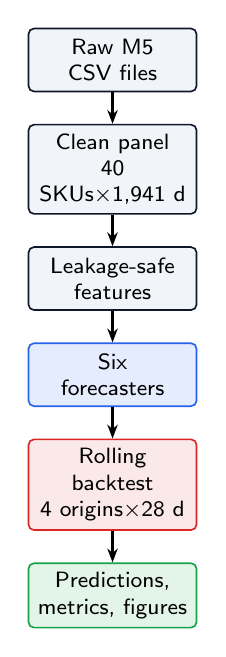
\begin{tikzpicture}[
  font=\sffamily\footnotesize, >={Stealth[length=5pt]}, node distance=4mm,
  blk/.style={draw, rounded corners=2pt, align=center, line width=0.6pt,
              minimum height=8mm, text width=19mm, fill=fcbg, draw=fcnavy},
]
\node[blk] (raw) {Raw M5\\CSV files};
\node[blk, below=of raw] (clean) {Clean panel\\40 SKUs$\times$1{,}941 d};
\node[blk, below=of clean] (feat) {Leakage-safe\\features};
\node[blk, below=of feat, fill=fcblue!12, draw=fcblue] (models) {Six\\forecasters};
\node[blk, below=of models, fill=fcred!10, draw=fcred] (bt) {Rolling backtest\\4 origins$\times$28 d};
\node[blk, below=of bt, fill=fcgreen!12, draw=fcgreen] (out) {Predictions,\\metrics, figures};
\draw[->, line width=0.8pt] (raw) -- (clean);
\draw[->, line width=0.8pt] (clean) -- (feat);
\draw[->, line width=0.8pt] (feat) -- (models);
\draw[->, line width=0.8pt] (models) -- (bt);
\draw[->, line width=0.8pt] (bt) -- (out);
\end{tikzpicture}
\caption{The forecasting pipeline. Notebook 01 produces the clean panel; notebook 02 builds
features, runs all six forecasters through the same backtest, and analyzes the results.}
\label{fig:pipeline}
\end{figure}

\subsection{Leakage-Safe Features}
\label{sec:features}
A feature is leakage-safe if its value on day $t$ depends only on sales up to day $t-1$ and the
calendar, which is published in advance. \Cref{tab:features} lists the features used by the
gradient-boosting and LSTM models. Lag features use \sig{shift(k)}; rolling means apply
\sig{shift(1)} before \sig{rolling(w)}, so the window for day $t$ covers days $t-w$ to $t-1$ and
never day $t$ itself. This property is tested, not assumed: one test perturbs sales after a cut-off
day and checks that earlier features are unchanged, and a second replaces every post-origin sale
with an out-of-range sentinel value and checks that no model's forecast changes -- both tests pass
\cite{kaufman2012}.

\begin{table}[t]
\centering
\caption{Leakage-Safe Features}
\label{tab:features}
\footnotesize
\begin{tabularx}{\columnwidth}{@{}l X@{}}
\toprule
Feature & Why it is there \\
\midrule
\sig{lag_1,7,14,28} & Autocorrelation peaks at 7, 14, 21, 28 days \\
\sig{roll_mean_7,28} & Recent level \\
\sig{dayofweek, is_weekend} & Weekend sales are 53\% above weekday \\
\sig{is_event, snap} & Known in advance; SNAP lifts sales $\approx$10\% \\
\sig{item_code} & Lets one pooled model learn per-SKU levels \\
\bottomrule
\end{tabularx}
\end{table}

\subsection{Baselines}
Seasonal naive with lag $m\in\{7,28\}$ repeats the observation from $m$ days earlier. It costs
nothing to compute and sets the bar a model must clear to be useful \cite{hyndman2021}.

\subsection{Pooled Gradient Boosting}
One scikit-learn histogram gradient-boosting regressor \cite{friedman2001} is trained on all
SKU-days before the origin (200 trees, learning rate 0.1, max depth 6, squared-error loss,
\sig{item_code} as a native categorical). Gradient boosting fits an additive ensemble of trees to
the negative loss gradient, which under squared error is the residual. Because lags beyond
$\tau{+}1$ are unknown at forecast time, the 28-day horizon is produced recursively: predict one
day, clip at zero, append it to the history, rebuild features, and repeat \cite{taieb2012}. This
keeps the model leakage-free but lets errors compound across the horizon.

\subsection{Local Kalman Filter}
\label{sec:kalman}
Each SKU is tracked by an independent linear-Gaussian state-space model with hidden state
$x_t=[\text{level}_t,\text{trend}_t]^\top$ (the \emph{local linear trend}, LLT, model):
\begin{equation}
  x_t = F x_{t-1} + w_t,\ w_t\sim\mathcal{N}(0,Q), \qquad
  y_t = H x_t + v_t,\ v_t\sim\mathcal{N}(0,R),
  \label{eq:ssm}
\end{equation}
with $F=\begin{psmallmatrix}1&1\\0&1\end{psmallmatrix}$ and $H=(1,0)$. A weekly-seasonal extension
(our addition beyond the base specification) appends six seasonal states constrained to sum to
roughly zero across the week, giving an 8-dimensional state that lets the filter learn a
day-of-week profile the plain LLT model cannot represent. \Cref{alg:kalman} is one predict/correct
cycle \cite{kalman1960}, implemented as shown in \cref{lst:kalman}.

\begin{algorithm}[t]
\caption{Kalman filter, one time step}
\label{alg:kalman}
\footnotesize
\begin{algorithmic}[1]
\State \textbf{Predict:} $\hat{x}\gets Fx$;\quad $\hat{P}\gets FPF^\top+Q$
\State \textbf{Innovation variance:} $S\gets H\hat{P}H^\top+R$
\State \textbf{Kalman gain:} $K\gets \hat{P}H^\top S^{-1}$
\State \textbf{Correct:} $x\gets \hat{x}+K(y-H\hat{x})$;\quad $P\gets (I-KH)\hat{P}$
\end{algorithmic}
\end{algorithm}

\begin{lstlisting}[caption={One predict/correct step (\texttt{kalman.py}).},label={lst:kalman},float=t]
def update(self, y):
    x_pred = self.F @ self.x
    P_pred = self.F @ self.P @ self.F.T + self.Q
    S = self.H @ P_pred @ self.H.T + self.R
    K = P_pred @ self.H.T / S
    self.x = x_pred + (K * (y - self.H @ x_pred)).ravel()
    self.P = (np.eye(len(self.x)) - K @ self.H) @ P_pred
\end{lstlisting}

Noise is set by a fixed rule rather than maximum likelihood: $R$ is the variance of the last 365
training days around their weekday means (floor $0.1$), and $Q$ is a small fixed fraction of $R$
on each state. To forecast $h$ steps ahead, the predict step is applied $h$ times with no further
corrections; the resulting variance grows with $h$, and the 80\% interval is the forecast mean
$\pm1.2816\sqrt{V(h)}$, clipped at zero. Fitting $Q,R$ by maximum likelihood \cite{durbin2012} would
likely narrow this interval; the fixed rule was chosen to keep the local model simple and
transparent, at the cost shown in \cref{sec:results}.

\subsection{Global Quantile LSTM}
\label{sec:lstm}
One LSTM \cite{hochreiter1997} is trained on all 40 SKUs jointly at every origin. For each SKU and
forecast start $t$, the network reads the previous 56 days of sales, scaled per \cref{eq:scale} in
the manner of DeepAR \cite{salinas2020} so that large and small SKUs look alike:
\begin{equation}
  \kappa_i = 1+\frac{1}{56}\sum_{j=t-56}^{t-1} y_{i,j}, \qquad s_{i,j} = y_{i,j}/\kappa_i .
  \label{eq:scale}
\end{equation}
Each input step also carries five calendar covariates (sine/cosine of day-of-week, weekend, event
and SNAP flags). An LSTM with hidden size 32 encodes the window; its final hidden state is
concatenated with a 4-dimensional learned SKU embedding and the flattened covariates of the 28
forecast days (176 inputs total) and passed through a two-layer perceptron
($176\to64\to84$, ReLU) to a $28\times3$ matrix of scaled quantiles (\cref{lst:lstm}), following the
direct multi-horizon design of MQ-RNN \cite{wen2017} rather than DeepAR's autoregressive sampling.
The model has 22{,}068 trainable parameters.

\begin{lstlisting}[caption={Forward pass (\texttt{global\_model.py}).},label={lst:lstm},float=t]
def forward(self, past, future_cov, item):
    _, (h, _) = self.lstm(past)
    parts = [h[-1], self.embedding(item),
             future_cov.flatten(1)]
    out = self.head(torch.cat(parts, dim=1))
    return out.view(-1, self.horizon, self.n_outputs)
\end{lstlisting}

Training minimizes pinball loss, \cref{eq:pinball}, averaged over the three quantiles
$\alpha\in\{0.1,0.5,0.9\}$ and all 28 horizon days:
\begin{equation}
  \rho_\alpha(u) = \max(\alpha u,\ (\alpha-1)u), \qquad u = y-q .
  \label{eq:pinball}
\end{equation}
At $\alpha=0.9$, under-forecasting is penalized nine times more heavily than over-forecasting.
Outputs are rescaled by $\kappa_i$, sorted so that $\mathrm{P10}\le\mathrm{P50}\le\mathrm{P90}$
\cite{chernozhukov2010}, and clipped at zero; $\mathrm{P50}$ is the point forecast. Training uses
Adam \cite{kingma2015} (learning rate $10^{-3}$, batch size 256, at most 20 epochs, early stopping
with patience 3) with no dropout or weight decay; the only regularizer is early stopping.

\subsection{Pinball Loss Minimizes a Quantile, Not a Mean}
\label{sec:prop}
\begin{definition}
For a point forecast $q$ of a random variable $Y$ with cumulative distribution function $F_Y$, the
\emph{pinball risk} at level $\alpha\in(0,1)$ is $R_\alpha(q)=\mathbb{E}[\rho_\alpha(Y-q)]$ with
$\rho_\alpha$ as in \cref{eq:pinball}.
\end{definition}
\begin{proposition}\label{prop:quantile}
If $F_Y$ is continuous at $q$, $R_\alpha(q)$ is minimized at $q^\star$ satisfying
$F_Y(q^\star)=\alpha$, i.e.\ $q^\star=F_Y^{-1}(\alpha)$, the $\alpha$-quantile of $Y$
\cite{koenker1978}.
\end{proposition}
\begin{proof}[Proof sketch]
The subgradient of $R_\alpha$ at $q$ is $\alpha-F_Y(q)$; setting it to zero gives
$F_Y(q^\star)=\alpha$.
\end{proof}
\begin{corollary}\label{cor:median}
At $\alpha=0.5$, $\rho_{0.5}(u)=\tfrac12|u|$, so $R_{0.5}$ is minimized by the \emph{median} of $Y$;
the squared-error loss used by gradient boosting and the Kalman filters is minimized by the
\emph{mean} of $Y$ \cite{kolassa2020}. The LSTM's P50 output and the other models' point forecasts
therefore target different statistics of the same demand distribution, which on zero-heavy, skewed
count data need not coincide.
\end{corollary}
\Cref{cor:median} is used in \cref{sec:results} to separate how much of the LSTM's advantage on
MAE/WAPE (both minimized by the median) reflects this choice of statistic rather than skill.

\subsection{Evaluation Protocol}
Four forecast origins, 28 days apart, cover the last 112 days of the panel (\cref{tab:origins}). At
each origin every model is refit on data strictly before the origin and forecasts the next 28 days
for all 40 SKUs; a fairness check confirms all six models are scored on identical origin, date, SKU
and actual rows.

\begin{table}[t]
\centering
\caption{Rolling Forecast Origins}
\label{tab:origins}
\footnotesize
\begin{tabular}{@{}c l c l@{}}
\toprule
Origin & Train until & Train days & Forecast window \\
\midrule
1 & 2016-01-31 & 1{,}829 & 2016-02-01 -- 02-28 \\
2 & 2016-02-28 & 1{,}857 & 2016-02-29 -- 03-27 \\
3 & 2016-03-27 & 1{,}885 & 2016-03-28 -- 04-24 \\
4 & 2016-04-24 & 1{,}913 & 2016-04-25 -- 05-22 \\
\bottomrule
\end{tabular}
\end{table}

SKUs with fewer than 56 days of selling history at the origin receive a cold-start fallback (the
median same-weekday sales of established SKUs over the last 28 days); none of the 40 SKUs triggers
this rule on real data, so it is exercised only by a synthetic unit test. \Cref{tab:metrics} lists
the accuracy and calibration metrics used in \cref{sec:results} \cite{hyndman2006}.

\begin{table}[t]
\centering
\caption{Evaluation Metrics}
\label{tab:metrics}
\footnotesize
\begin{tabularx}{\columnwidth}{@{}l X@{}}
\toprule
Metric & Definition \\
\midrule
MAE & Mean $|y-\hat{y}|$; minimized by the median \\
RMSE & $\sqrt{\text{mean}(y-\hat{y})^2}$; minimized by the mean \\
$\WAPE$ & $\sum|y-\hat{y}|/\sum y$; well-defined when individual $y{=}0$ \\
Pinball & $\rho_\alpha(y-\hat{q})$ at $\alpha=0.1,0.5,0.9$ \\
Coverage & Share of $y$ inside $[\mathrm{P10},\mathrm{P90}]$; target $0.80$ \\
\bottomrule
\end{tabularx}
\end{table}

\subsection{Design Decisions Not Taken}
A DeepAR model with a negative-binomial likelihood would likely fit count data better than a
Gaussian Kalman filter or a direct quantile head, but was left for future work to limit integration
risk. Maximum-likelihood noise estimation for the Kalman filter, Croston-type intermittent-demand
baselines \cite{croston1972,syntetos2005}, a tuned or count-aware boosting objective, and
attention-based architectures \cite{lim2021} were all considered and set aside for the same reason:
each adds a design axis this controlled comparison was not built to vary.

% =============================================================================
\section{Results and Discussion}
\label{sec:results}
% =============================================================================

\subsection{Overall Accuracy}
\Cref{tab:results} reports pooled metrics over all 40 SKUs, 4 origins and 28 days (4{,}480
SKU-days per model). The global LSTM leads on every metric; only it and gradient boosting beat the
lag-7 naive baseline.

\begin{table}[t]
\centering
\caption{Pooled Accuracy and Calibration}
\label{tab:results}
\footnotesize
\begin{tabular}{@{}l c c c c@{}}
\toprule
Model & MAE & RMSE & $\WAPE$ & Coverage \\
\midrule
Global LSTM (quantile) & \textbf{1.555} & \textbf{3.533} & \textbf{0.499} & \textbf{0.812} \\
Gradient boosting & 1.763 & 3.672 & 0.566 & n/a \\
Seasonal naive (lag-7) & 1.940 & 4.310 & 0.623 & n/a \\
Seasonal naive (lag-28) & 1.992 & 4.511 & 0.639 & n/a \\
Kalman (+weekly) & 2.108 & 5.025 & 0.676 & 0.950 \\
Kalman (level+trend) & 2.445 & 6.475 & 0.785 & 0.945 \\
\bottomrule
\end{tabular}
\end{table}

\begin{figure}[t]
\centering
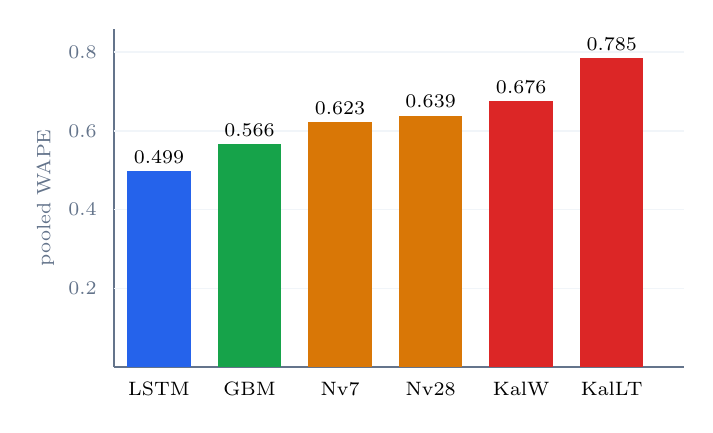
\begin{tikzpicture}[x=1.15cm,y=5cm]
  \draw[fcslate, line width=0.6pt] (0,0) -- (6.3,0);
  \draw[fcslate, line width=0.6pt] (0,0) -- (0,0.86);
  \foreach \gy in {0.2,0.4,0.6,0.8} {
    \draw[fcbg, line width=0.5pt] (0,\gy) -- (6.3,\gy);
    \node[anchor=east, font=\scriptsize, text=fcslate] at (-0.08,\gy) {\gy};
  }
  \node[rotate=90, anchor=south, font=\scriptsize, text=fcslate] at (-0.55,0.43) {pooled WAPE};
  \foreach \x/\v/\c/\l in {%
    0.5/0.499/fcblue/LSTM, 1.5/0.566/fcgreen/GBM, 2.5/0.623/fcamber/Nv7,
    3.5/0.639/fcamber/Nv28, 4.5/0.676/fcred/KalW, 5.5/0.785/fcred/KalLT} {
    \fill[\c] (\x-0.35,0) rectangle (\x+0.35,\v);
    \node[font=\scriptsize] at (\x,\v+0.035) {\v};
    \node[anchor=north, font=\scriptsize, yshift=-2pt] at (\x,0) {\l};
  }
\end{tikzpicture}
\caption{Pooled WAPE by model (lower is better). LSTM: global quantile LSTM; GBM: gradient
boosting; Nv7/Nv28: seasonal naive lag 7/28; KalW/KalLT: Kalman with/without weekly seasonality.}
\label{fig:wape-bar}
\end{figure}

Adding weekly seasonality improves the Kalman filter's $\WAPE$ from 0.785 to 0.676
(\cref{fig:wape-bar}), confirming that the weekly cycle found in exploratory analysis is the
dominant structure the plain local-linear-trend model misses -- yet even the improved filter never
catches the naive baselines.

\subsection{Stability Across Origins and Forecast Horizon}
The LSTM's $\WAPE$ varies only between 0.478 and 0.520 across the four origins, while gradient
boosting beats lag-7 naive at three of four and both Kalman filters spike at origin 3 (traced to a
single SKU in \cref{sec:case}). \Cref{fig:horizon} breaks accuracy down by week of the 28-day
horizon: the local Kalman filter is the only model that looks competitive anywhere, beating both
naive baselines in the first week (0.567 against 0.635/0.644), then degrading steadily to 0.786 by
the final week, because it extrapolates its last level and trend with no knowledge of the future
calendar. The LSTM and gradient boosting, which both condition on the known future calendar, stay
nearly flat across the horizon.

\begin{figure}[t]
\centering
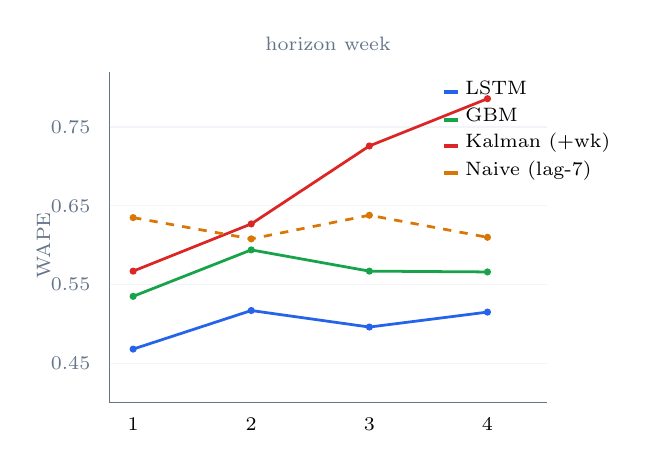
\begin{tikzpicture}[x=1.5cm,y=10cm]
  \draw[fcslate, line width=0.6pt] (0.8,0.4) -- (4.5,0.4);
  \draw[fcslate, line width=0.6pt] (0.8,0.4) -- (0.8,0.82);
  \foreach \gy in {0.45,0.55,0.65,0.75} {
    \draw[fcbg, line width=0.5pt] (0.8,\gy) -- (4.5,\gy);
    \node[anchor=east, font=\scriptsize, text=fcslate] at (0.72,\gy) {\gy};
  }
  \foreach \gx in {1,2,3,4} {
    \node[anchor=north, font=\scriptsize, yshift=-2pt] at (\gx,0.4) {\gx};
  }
  \node[anchor=south, font=\scriptsize, text=fcslate] at (2.65,0.835) {horizon week};
  \node[rotate=90, anchor=south, font=\scriptsize, text=fcslate] at (0.38,0.6) {WAPE};
  \draw[fcblue, line width=1pt] plot coordinates {(1,0.468) (2,0.517) (3,0.496) (4,0.515)};
  \foreach \px/\py in {1/0.468,2/0.517,3/0.496,4/0.515} {\fill[fcblue] (\px,\py) circle (1.3pt);}
  \draw[fcgreen, line width=1pt] plot coordinates {(1,0.535) (2,0.594) (3,0.567) (4,0.566)};
  \foreach \px/\py in {1/0.535,2/0.594,3/0.567,4/0.566} {\fill[fcgreen] (\px,\py) circle (1.3pt);}
  \draw[fcred, line width=1pt] plot coordinates {(1,0.567) (2,0.627) (3,0.726) (4,0.786)};
  \foreach \px/\py in {1/0.567,2/0.627,3/0.726,4/0.786} {\fill[fcred] (\px,\py) circle (1.3pt);}
  \draw[fcamber, line width=1pt, dashed] plot coordinates {(1,0.635) (2,0.608) (3,0.638) (4,0.610)};
  \foreach \px/\py in {1/0.635,2/0.608,3/0.638,4/0.610} {\fill[fcamber] (\px,\py) circle (1.3pt);}
  \node[anchor=west, font=\scriptsize] at (3.55,0.80) {\textcolor{fcblue}{\rule{5pt}{1.4pt}} LSTM};
  \node[anchor=west, font=\scriptsize] at (3.55,0.765) {\textcolor{fcgreen}{\rule{5pt}{1.4pt}} GBM};
  \node[anchor=west, font=\scriptsize] at (3.55,0.73) {\textcolor{fcred}{\rule{5pt}{1.4pt}} Kalman (+wk)};
  \node[anchor=west, font=\scriptsize] at (3.55,0.695) {\textcolor{fcamber}{\rule{5pt}{1.4pt}} Naive (lag-7)};
\end{tikzpicture}
\caption{WAPE by week of the 28-day forecast horizon. The Kalman filter is competitive only in the
first week; the LSTM and gradient boosting stay flat because both see the future calendar.}
\label{fig:horizon}
\end{figure}

\subsection{Error by Demand Class}
\Cref{tab:class} shows every model struggles on lumpy SKUs, where every model except the LSTM scores
a WAPE above 1.0 -- worse than forecasting zero every day. The intermittent class's low pooled WAPE
is driven largely by \texttt{FOODS\_3\_090}, which supplies 64.9\% of that class's test volume.

\begin{table}[t]
\centering
\caption{WAPE by Demand Class (Share of Test Volume)}
\label{tab:class}
\footnotesize
\begin{tabular}{@{}l c c c c@{}}
\toprule
Model & Smooth & Erratic & Intermit. & Lumpy \\
 & (17.0\%) & (4.2\%) & (66.1\%) & (12.6\%) \\
\midrule
Global LSTM & \textbf{0.574} & \textbf{0.540} & \textbf{0.412} & \textbf{0.839} \\
Gradient boosting & 0.592 & 0.552 & 0.475 & 1.008 \\
Kalman (+weekly) & 0.736 & 0.686 & 0.578 & 1.106 \\
Naive (lag-7) & 0.759 & 0.710 & 0.493 & 1.088 \\
\bottomrule
\end{tabular}
\end{table}

\subsection{Per-SKU Results and Volume Concentration}
At the level of single SKUs, the LSTM has the lowest MAE on 31 of 40 SKUs, gradient boosting on 5,
the weekly Kalman filter on 3, and the plain Kalman filter on 1. Removing \texttt{FOODS\_3\_090}
entirely leaves the ranking unchanged (LSTM 0.677, gradient boosting 0.789, lag-7 naive 0.879,
weekly Kalman 0.906, LLT Kalman 0.976), so the pooled result in \cref{tab:results} is not an
artifact of one high-volume series.

\subsection{Case Study: Trend Extrapolation Fails at Origin 3}
\label{sec:case}
At origin 3 the local-linear-trend filter forecast 2{,}878 units of \texttt{FOODS\_3\_090} over 28
days against 1{,}423 actual -- a 102\% over-forecast; at the other three origins its totals were
within 15\%--39\% of actual. A short run of high sales before the origin pushed the trend state up;
because each forecast step adds the trend unchanged, the over-forecast grows linearly across the
month. Retail demand rarely sustains a linear drift for 28 days, which is the structural reason a
damped-trend or trend-free local model would be a direct fix.

\subsection{Seed Stability}
Repeating the full four-origin LSTM backtest with three random seeds gives
$\WAPE=0.501\pm0.003$, $\mathrm{MAE}=1.560\pm0.011$ and coverage $0.816\pm0.003$ (mean $\pm$
standard deviation). Even the worst seed ($\WAPE=0.504$) beats gradient boosting by 0.062,
confirming the ranking is not a training-noise artifact.

\subsection{Calibration}
The LSTM's 80\% interval covers 81.2\% of outcomes pooled, and between 77.8\% (lumpy) and 86.6\%
(erratic) by demand class. Both Kalman filters over-cover in every class (0.938--0.954) by quoting
intervals 1.8--1.9 times wider (10.60--11.11 units against 5.98), which in inventory terms means
carrying excess safety stock to achieve a coverage the model did not need to promise.
\Cref{fig:panel} illustrates this directly: panel (a) is the headline model-comparison chart,
panel (b) is the per-SKU WAPE distribution underlying \cref{tab:results}, and panel (c) shows the
Kalman interval widening with horizon regardless of the data, against the LSTM's interval tracking
the weekly pattern.

\begin{figure*}[t]
\centering
\subfloat[Pooled WAPE by model (bar chart recreated from \texttt{outputs/metrics.csv}).]{%
  \safeimage{0.31\textwidth}{../outputs/figures/11_model_comparison.png}}\hfill
\subfloat[Distribution of per-SKU WAPE, all six models.]{%
  \safeimage{0.31\textwidth}{../outputs/figures/13_per_sku_wape.png}}\hfill
\subfloat[P10--P90 uncertainty bands, Kalman filter versus LSTM, one SKU.]{%
  \safeimage{0.31\textwidth}{../outputs/figures/17_uncertainty_bands.png}}
\caption{Supporting figures generated by \texttt{notebooks/02\_model\_comparison.ipynb} from
\texttt{outputs/predictions.csv} and \texttt{outputs/metrics.csv}.}
\label{fig:panel}
\end{figure*}

\subsection{What the Results Do Not Show}
By \cref{cor:median}, the LSTM's point forecast is a conditional median and every other model's is
a conditional mean. The median minimizes absolute error, so part of the LSTM's MAE/WAPE lead
reflects the statistic being forecast rather than pure skill. This cannot be the whole explanation,
however: the LSTM also wins on RMSE, which rewards the mean, but by a smaller margin (3.533 against
3.672), so a real accuracy gap remains after accounting for the choice of statistic. No formal
significance test (e.g.\ Diebold--Mariano \cite{diebold1995}) was run; the lead holding across
origins, demand classes, horizon weeks, 31 of 40 SKUs, three seeds, and the SKU-exclusion check is
strong informal evidence that a formal test would very likely confirm.

\subsection{Summary Against the Research Questions}
\Cref{tab:objectives} maps each research question from \cref{sec:background} to the evidence
presented above.

\begin{table}[t]
\centering
\caption{Research Questions and Supporting Evidence}
\label{tab:objectives}
\footnotesize
\begin{tabularx}{\columnwidth}{@{}>{\raggedright\arraybackslash}p{0.4\columnwidth} X@{}}
\toprule
Question & Evidence \\
\midrule
Does a global model beat local/naive models? & Yes: \cref{tab:results,fig:wape-bar}; robust to seed
  and SKU exclusion (\S\ref{sec:results}) \\
When does the local Kalman filter stay competitive? & Only in horizon week 1, and only against
  naive baselines (\cref{fig:horizon}) \\
How well calibrated are the quantile forecasts? & LSTM near-nominal (0.812 vs.\ 0.80 target);
  Kalman over-covers via wide intervals (\S\ref{sec:results}F) \\
\bottomrule
\end{tabularx}
\end{table}

\subsection{Threats to Validity}
The comparison covers one store, one category, 40 SKUs and four consecutive 28-day windows from
February to May 2016; it may not transfer to other stores, categories or seasons. No model was
tuned, so gradient boosting's 0.067 WAPE gap to the LSTM is best read as an upper bound on the
LSTM's advantage over well-engineered tabular learning, not a ceiling. The Kalman filter's noise
parameters come from a fixed rule rather than maximum likelihood, which likely inflates its
intervals beyond what a better-fit filter would need. Croston-type intermittent-demand baselines
were not included despite 22 of 40 SKUs being intermittent. The raw data came from a third-party
mirror whose shapes match the official Kaggle release; checksums were not compared.

% =============================================================================
\section{Conclusion}
\label{sec:conclusion}
% =============================================================================
Six forecasters -- two naive baselines, pooled gradient boosting, two per-SKU Kalman filters, and a
global quantile LSTM -- were compared under one leakage-tested rolling backtest on 40 M5 SKUs. The
global LSTM is the most accurate and the best-calibrated model by every measure used, and its
advantage is robust across forecast origins, demand classes, horizon weeks, individual SKUs, random
seeds, and the removal of the single highest-volume series. The local Kalman filter is competitive
only in the first forecast week and only against naive baselines; a case study traces its worst
failure to trend extrapolation from a short sales spike, and its nominal 80\% coverage is bought
with intervals nearly twice as wide as the LSTM's. A formal decomposition shows that part of the
LSTM's lead on MAE and WAPE reflects its forecasting a median rather than a mean, though a
real accuracy gap remains after accounting for this. Future work could add a DeepAR-style
negative-binomial head, Croston/SBA baselines for the intermittent SKUs, maximum-likelihood Kalman
noise with a damped trend, a formal Diebold--Mariano significance test, and a hybrid model that
feeds Kalman state estimates into the LSTM as extra inputs.

% =============================================================================
\section*{Author Contributions}
% =============================================================================
\noindent{\footnotesize
\begin{tabularx}{\columnwidth}{@{}l X@{}}
\toprule
Author & Primary responsibility \\
\midrule
Sayan Bhattacharya & Data-cleaning pipeline \\
Aryu Rao & Demand classification and data audit \\
Debasish Karan & Feature engineering \\
Saswataduity Bhuin & Exploratory data analysis \\
Aryan Vibhuti & Model training \\
\bottomrule
\end{tabularx}}

\vspace{4pt}\noindent All authors contributed to the backtest design, the analysis of results, and
approved the final manuscript.

\begin{thebibliography}{99}

\bibitem{makridakis2022} S. Makridakis, E. Spiliotis, and V. Assimakopoulos, ``M5 accuracy
  competition: Results, findings, and conclusions,'' \emph{Int. J. Forecasting}, vol.~38, no.~4,
  pp.~1346--1364, 2022. doi: 10.1016/j.ijforecast.2021.11.013.

\bibitem{montero2021} P. Montero-Manso and R. J. Hyndman, ``Principles and algorithms for
  forecasting groups of time series: Locality and globality,'' \emph{Int. J. Forecasting}, vol.~37,
  no.~4, pp.~1632--1653, 2021. doi: 10.1016/j.ijforecast.2021.03.004.

\bibitem{hyndman2021} R. J. Hyndman and G. Athanasopoulos, \emph{Forecasting: Principles and
  Practice}, 3rd ed. OTexts, 2021. [Online]. Available: \url{https://otexts.com/fpp3/}.

\bibitem{salinas2020} D. Salinas, V. Flunkert, J. Gasthaus, and T. Januschowski, ``DeepAR:
  Probabilistic forecasting with autoregressive recurrent networks,'' \emph{Int. J. Forecasting},
  vol.~36, no.~3, pp.~1181--1191, 2020. doi: 10.1016/j.ijforecast.2019.07.001.

\bibitem{wen2017} R. Wen, K. Torkkola, B. Narayanaswamy, and D. Madeka, ``A multi-horizon quantile
  recurrent forecaster,'' arXiv:1711.11053, 2017.

\bibitem{friedman2001} J. H. Friedman, ``Greedy function approximation: A gradient boosting
  machine,'' \emph{Ann. Statist.}, vol.~29, no.~5, pp.~1189--1232, 2001. doi:
  10.1214/aos/1013203451.

\bibitem{taieb2012} S. Ben Taieb, G. Bontempi, A. F. Atiya, and A. Sorjamaa, ``A review and
  comparison of strategies for multi-step ahead time series forecasting based on the NN5 forecasting
  competition,'' \emph{Expert Syst. Appl.}, vol.~39, no.~8, pp.~7067--7083, 2012. doi:
  10.1016/j.eswa.2012.01.039.

\bibitem{kalman1960} R. E. Kalman, ``A new approach to linear filtering and prediction problems,''
  \emph{J. Basic Eng.}, vol.~82, no.~1, pp.~35--45, 1960. doi: 10.1115/1.3662552.

\bibitem{hochreiter1997} S. Hochreiter and J. Schmidhuber, ``Long short-term memory,'' \emph{Neural
  Comput.}, vol.~9, no.~8, pp.~1735--1780, 1997. doi: 10.1162/neco.1997.9.8.1735.

\bibitem{koenker1978} R. Koenker and G. Bassett, Jr., ``Regression quantiles,'' \emph{Econometrica},
  vol.~46, no.~1, pp.~33--50, 1978. doi: 10.2307/1913643.

\bibitem{gneiting2007} T. Gneiting and A. E. Raftery, ``Strictly proper scoring rules, prediction,
  and estimation,'' \emph{J. Amer. Statist. Assoc.}, vol.~102, no.~477, pp.~359--378, 2007. doi:
  10.1198/016214506000001437.

\bibitem{kingma2015} D. P. Kingma and J. Ba, ``Adam: A method for stochastic optimization,'' in
  \emph{Proc. ICLR}, 2015. arXiv:1412.6980.

\bibitem{chernozhukov2010} V. Chernozhukov, I. Fern\'andez-Val, and A. Galichon, ``Quantile and
  probability curves without crossing,'' \emph{Econometrica}, vol.~78, no.~3, pp.~1093--1125, 2010.
  doi: 10.3982/ECTA7880.

\bibitem{kaufman2012} S. Kaufman, S. Rosset, and C. Perlich, ``Leakage in data mining: Formulation,
  detection, and avoidance,'' \emph{ACM Trans. Knowl. Discov. Data}, vol.~6, no.~4, pp.~1--21, 2012.
  doi: 10.1145/2382577.2382579.

\bibitem{tashman2000} L. J. Tashman, ``Out-of-sample tests of forecasting accuracy: An analysis and
  review,'' \emph{Int. J. Forecasting}, vol.~16, no.~4, pp.~437--450, 2000. doi:
  10.1016/S0169-2070(00)00065-0.

\bibitem{hyndman2006} R. J. Hyndman and A. B. Koehler, ``Another look at measures of forecast
  accuracy,'' \emph{Int. J. Forecasting}, vol.~22, no.~4, pp.~679--688, 2006. doi:
  10.1016/j.ijforecast.2006.03.001.

\bibitem{durbin2012} J. Durbin and S. J. Koopman, \emph{Time Series Analysis by State Space
  Methods}, 2nd ed. Oxford, U.K.: Oxford Univ. Press, 2012.

\bibitem{croston1972} J. D. Croston, ``Forecasting and stock control for intermittent demands,''
  \emph{Oper. Res. Q.}, vol.~23, no.~3, pp.~289--303, 1972. doi: 10.1057/jors.1972.50.

\bibitem{syntetos2005} A. A. Syntetos and J. E. Boylan, ``On the categorization of demand
  patterns,'' \emph{J. Oper. Res. Soc.}, vol.~56, no.~5, pp.~495--503, 2005. doi:
  10.1057/palgrave.jors.2601841.

\bibitem{lim2021} B. Lim, S. {\"O}. Ar\i k, N. Loeff, and T. Pfister, ``Temporal fusion transformers
  for interpretable multi-horizon time series forecasting,'' \emph{Int. J. Forecasting}, vol.~37,
  no.~4, pp.~1748--1764, 2021. doi: 10.1016/j.ijforecast.2021.03.012.

\bibitem{kolassa2020} S. Kolassa, ``Why the ``best'' point forecast depends on the error or
  accuracy measure,'' \emph{Int. J. Forecasting}, vol.~36, no.~1, pp.~208--211, 2020. doi:
  10.1016/j.ijforecast.2019.02.017.

\bibitem{diebold1995} F. X. Diebold and R. S. Mariano, ``Comparing predictive accuracy,'' \emph{J.
  Bus. Econ. Statist.}, vol.~13, no.~3, pp.~253--263, 1995. doi: 10.1080/07350015.1995.10524599.

\end{thebibliography}

\end{document}
